\lab{Python}{Data Structures}{Data Structures}
\label{lab:Python_DataStructures}
\objective{Empower students with basic knowledge of the fundamental, canonical data structures in order to understand performance and runtime characteristics.}

Both storing and retrieving data take time. As the size of a data set grows, the time it takes to manipulate the set also grows accordingly (be that growth logarithmic, linear, exponential, or factorial).
The overhead associated with working with large data sets makes it crucial that we have a fundamental knowledge of the data structures used to store them.
As we understand the characteristics of such data structures, we will be able to choose the data structure that will help us to most efficiently access the data that we need.

\section*{Abstract Data Types}

The most basic way to store data is via \emph{primitive data types}.
These data types are booleans, strings, floats, and integers.
Most information that we care to store is in one of these forms; however, these primitive types can quickly become unwieldy for storing large amounts of information.
Imagine having a different name for every piece of data you use!
Luckily, we can create more natural ways to store data by using primitive data types, along with arrays, as our building blocks.
In object oriented progamming, for example, we often use these ``building blocks'' to create the various classes we require.
More complex data structures are called \emph{abstract data types}.
Python possesses a couple of the more common abstract data types, including dictionaries, sets, and lists.
However, the performance of each abstract data types slows down as the size of the data structure increases.

Most abstract data types use an object called a \emph{node} to store data.
A node essentially acts as a box in which we store an arbitrary piece of data.
Nodes can store absolutely anything; what they contain both depends on the data structure itself and data that is actually being stored.
A good way to understand an abstract data structure is to think of it like the postal delivery system.
We start by inserting an item into the postal system.
(Because the data stored in a node is arbitrary, our item can be anything.)
The first thing that the postal system will do with our item is put it into a box and attach delivery specific data that would allow it to be processed more effectively, like the return address or a little label indicating that the contents are ``fragile.''
The postal system now only has to efficiently handle boxes; it doesn't have to worry about working with each item that goes through system.
Thus, the postal system has abstracted itself from the items it delivers.

If we didn't use nodes or ``data boxes'', we would have to build a new structure for each data type we wanted to store.
Thus, nodes allow us to abstract the data structure from the kind of data we stored inside.
Nodes allow us to generalize the functionality of a data structure.

\section*{Linked Lists}
\emph{Linked lists} are one of the most fundamental of the basic data structures.
A linked list, in essence, is simply a list of nodes that are linked together.
There are three common types of linked lists: singly-linked, \ref{Singly-linked List}; doubly-linked, \ref{Doubly-linked List}; and circularly-linked, \ref{Circularly-linked List}.

\begin{figure}[!h]
\centering
\begin{tikzpicture}[->,>=stealth',shorten >=1pt,auto, node distance=1.5cm,
  thick,main node/.style={rectangle,draw}, minimum size=.5cm]
\tikzset{rect node/.style={rectangle, draw, minimum height = .5cm, minimum width=.2cm}}
  \node[main node] (1) {B};
  \node[main node] (2) [right of=1] {F};
  \node[main node] (3) [right of=2] {G};
  \node[main node] (4) [right of=3] {C};
  \node[draw = none, black!20!blue, node distance=1.5cm] [above left of=1](H) {Head};
  \node[rect node][right of=1, node distance = .36cm]{};
  \node[rect node][right of=2, node distance = .36cm]{};
  \node[rect node][right of=3, node distance = .36cm]{};
  \node[rect node](5)[right of=4, node distance = .36cm]{};
  \node[draw = none, node distance = 1.5cm] [right of=4]{};  % Centralize this particular figure
\foreach \s/\t  in {1/2, 2/3, 3/4}{
	\path[draw](\s) edge[shorten <=.1cm](\t);}

  \draw[black!20!blue] (H) edge (1.north);
\end{tikzpicture}
\caption{Singly-linked List}
\label{Singly-linked List}
\end{figure}

A singly-linked node stores a piece of data (its value), and a single reference that points to the next node in the list.
We implement a singly-linked node class as follows:

\begin{lstlisting}
class Node():
    def __init__(self):
        self.next = None
        self.value = None
\end{lstlisting}

\begin{figure}[!h]
\centering
\begin{tikzpicture}[->,>=stealth',shorten >=1pt,auto, node distance=1.5cm,
  thick,main node/.style={rectangle,draw}, minimum size=.5cm]
\tikzset{rect node/.style={rectangle, draw, minimum height = .5cm, minimum width=.9cm}}
  \node[main node] (1) {B};
  \node[main node] (2) [right of=1] {F};
  \node[main node] (3) [right of=2] {G};
  \node[main node] (4) [right of=3] {C};
  \node[draw = none, black!20!blue, node distance = 1.5cm] [above right of=4] (T) {Tail};
  \node[draw = none, black!20!blue, node distance = 1.5cm] [above left of=1] (H) {Head};
  \node[rect node](1.5)[]{};
  \node[rect node](2.5)[right of=1.5]{};
  \node[rect node](3.5)[right of=2.5]{};
  \node[rect node](4.5)[right of=3.5]{};

\foreach \s/\t  in {1/2, 2/3, 2/1, 3/2, 3/4, 4/3}{
	\path[draw](\s) edge[shorten <=.1cm, shorten >=.1cm](\t);}
	

  \draw[black!20!blue] (H) edge (1.north);
  \draw[black!20!blue] (T) edge (4.north);
\end{tikzpicture}
\caption{Doubly-linked List}
\label{Doubly-linked List}
\end{figure}

Doubly-linked nodes have two references: one that points to the previous node and one that points to the next node in the list.
This allows for a doubly-linked list to be traversed in both directions, whereas a singly-linked list can only be traversed in one direction.
We modify our node, then, to allow for a reference to the previous node.

\begin{lstlisting}
class Node():
    def __init__(self):
        self.next = None
        self.previous = None
        self.value = None
\end{lstlisting}

\begin{figure}[!h]
\centering
\begin{tikzpicture}[->,>=stealth',shorten >=1pt,auto, node distance=1.5cm,
  thick,main node/.style={rectangle,draw}, minimum size=.5cm]
\tikzset{rect node/.style={rectangle, draw, minimum height = .5cm, minimum width=.2cm}}

   \node[main node] (1) {B};
  \node[main node] (2) [right of=1] {F};
  \node[main node] (3) [right of=2] {G};
  \node[main node] (4) [right of=3] {C};
  \node[](H) [above of=1, node distance = 1.5cm, color = black!20!blue] {Head};
  \node[rect node][right of=1, node distance = .36cm]{};
  \node[rect node][right of=2, node distance = .36cm]{};
  \node[rect node][right of=3, node distance = .36cm]{};
  \node[rect node](5)[right of=4, node distance = .36cm]{};

\foreach \s/\t  in {1/2, 2/3, 3/4}{
	\path[draw](\s) edge[shorten <=.1cm](\t);}

 \path[] (5.east) edge[out=60, in=30] node[right] {} (1.north);

  \path[black!20!blue]
     (H) edge node {}(1);
\end{tikzpicture}
\caption{Circularly, Singly-linked List}
\label{Circularly-linked List}
\end{figure}
A circularly-linked list is a linked list where the last node (the \emph{tail}) points to the first node (the \emph{head}) as its next node.
In a circularly, doubly-linked list, the head also points to the tail as its previous node.

We begin constructing our linked list class with a reference to the head node:
\begin{lstlisting}
class LinkedList():
    def __init__(self):
        self.head = None
\end{lstlisting}

Linked Lists may also have a reference to the tail node and a counter to keep track of the size of the list.
Including a tail reference allows us to avoid traversing the entire list each time we wish to insert at the end.
Similarly, though keeping a counter takes memory, without it we would have to recount the list every time we wanted to know its size.
\begin{lstlisting}
class LinkedList():
    def __init__(self):
        self.head = None
        self.tail = None
        self.counter = 0
    def size(self):
        return self.counter
\end{lstlisting}

\subsection*{Finding, Inserting and Removing}
Unlike arrays, which have random access, a linked list must walk through each node, starting with its single reference to the head, to find later ones in the list.
\begin{lstlisting}
    def find(self, data):
        tempnode = self.head
        while tempnode != None:
            if tempnode.value == data:
                return tempnode
            else:
                tempnode = tempnode.next
        # If tempnode == None, the method has traversed the list all the way to
        # the tail without finding a node corresponding to the data.
        return False
\end{lstlisting}
In order to insert or delete nodes found in the middle of the list, then, we must first locate the correct node by traversing the list - starting at the head and visiting each node.
Thus, nodes can be inserted or removed from either end of a linked list in constant time, independent of the size of the list, but inserting in and removing from the middle takes longer as the size of the list grows.
To insert into the end of a linked list, we need to make the old tail of the list reference the new node, increase the size counter, and update the reference to the tail of the list (if we choose to have either).

\begin{lstlisting}
    def insert(self, data):
        # Initialize a temporary node to store the desired piece of data.
        tempnode = Node()
        tempnode.value = data
        # If the linked list is empty, set the inserted piece of data as the
        # head node.
        if self.head == None:
            self.head = tempnode
        else:
            self.tail.next = tempnode
        # Update the existing tail node.
        self.tail = tempnode
        # Increase the size counter
        self.counter += 1
\end{lstlisting}

Removing a node involves a few additional considerations.
To remove a node from the middle of the list, we need to update the reference in the node before.
Furthermore, if we are removing a node from a doubly-linked list, we need to update the reference in the node after.
If we have a size counter, we also need to decrease the size counter to compensate for the removal.
To remove the last node in the list, we also need to update the reference to the tail, and, if it is the \emph{only} node in the list, we must set the reference to the head to \li{None}.

\begin{problem}
Implement a \li{remove(self, data)} method that will take a piece of data as its argument and remove its corresponding node form anywhere in the list.
Be sure to update your counter and references appropriately as you compensate for all possible situations (e.g. The data corresponds to none of the nodes in your linked list, your linked list consists of a single node, etc.)

The code below provides two additional methods to supplement your \li{LinkedList} class: one to clear the list and one to represent the list as a string.
These functions may be useful for testing your removal method.
\begin{lstlisting}
def clear(self):
    self.head = None
def __repr__(self):
    temp = self.head
    string = '['
    while temp != None:
        string += str(temp.value) + ','
        temp = temp.right
    string += ']'
    return string
\end{lstlisting}
\label{prob:LinkedLists}
\emph{Note}: Because Python is able to keep track of the variables we use, it will automatically delete a variable if there is no access to it.
In our \li{clear} method, this property allows us to set the reference to the head to be \li{None} which, in turn, allows Python to clean up the leftover nodes (in other languages, this might cause serious memory leaks).

\end{problem}

\section*{Stacks, Queues, and Deques}
\emph{Stacks}, \emph{queues} (pronounced `cue'), and \emph{deques} (pronounced `deck') can be thought of as types of linked lists where access is restricted.
Rather than accessing data anywhere in the list, we only add and remove from certain sides.
This means that rather than searching for a certain piece of data to remove we use them to keep track of the order the data was added in and simply ask for what is on the end.

Stacks are built on the in `last in, first out' principle, meaning that the last item that was put in the stack will be the first one to leave.
You can imagine this as a pile of plates in the kitchen cupboard. Rarely, if ever, do you take the plate on the bottom of the pile.
Instead you take the one on the top. Also, when putting plates in the cupboard, you put them on top of the pile.
This means that the last plate put in will be the first one taken out.
To implement this, we would only add and remove from the same side of a linked list.

Queues use `first in, first out,' meaning that the first thing put in will be the first thing taken out.
This is similar to people waiting in line.
The first person in line will be the first served and taken out of the line.
This is implemented as a linked list where we add on the right and remove on the left.

Deques are double ended queues, meaning that we can add and remove on either end.
Really the only difference between this and a linked list is that we cannot add and remove from the middle.

\begin{problem}
Implement a queue and a stack by having them inherit from your linked list class.
Have the stack add and remove from the right.
Have the queue add on the right and remove from the left.
\label{prob:Stack}
\end{problem}

\section*{Hash Tables}
A \emph{hash table} is a very simple data structure that trades space for speed.
Most of the operations of a hash table execute in constant time, independent of the size of the data structure.
As such, hash tables have very fast lookup times; they form the underlying data structure of Python's dictionaries.

In essence, a hash table is an array, but rather than walking through to look for our a piece of data, we have a \emph{hash function} that takes our data as an input and then outputs a positive integer used to index the array.
Since the hash function must be executed to perform any operation on the hash table, it is important that the hash function executes quickly.
Thus, the heart of a hash table is a good hash function.

What makes a good hash function?
Hash functions need to distribute items evenly throughout the hash table.
Since we usually mod by the table size at the end, we need to make sure the remainders mod $n$ are evenly distributed.
For example, if our hash function is the length of a string mod $n$, once the table gets large very few strings will be hashed to the end of the table.
We can fix this by multiplying by a large prime number.
A large number helps guarantee that the remainders will vary, and prime rids us of the chance that we are multiplying by a multiple of the table size (which would send us to 0 every time).

Let's walk through a simple example where we use a hash table to store strings.
Our hash function will be the length of the string mod the size of the table.
Thus, if our table has size 4, `cat' would be stored in spot 3.
Similarly, `lion' would be sent to 4 \% 4 = 0.
\[
\begin{tabular}{|c|c|c|c|}
\hline
0 & 1 & 2 & 3\\
\hline
`lion' & & & `cat' \\
\hline
\end{tabular}
\]


\begin{problem}
Implement a hash table to store tuples of names and i.d.s with methods to add and remove items.
Implement it so that when a hash table object is created, you pass in a parameter to specify the size.
Have your hash function take the i.d., multiply by 7927 (a prime number), and mod by the size of the table.
\label{prob:Hash1}
\end{problem}

In our earlier example, our hash function is far from perfect.
If we try to store `leopard', our hash function sends it to 7 \% 4 = 3.
But `cat' is already stored in spot 3.
This is called a \emph{hash collision}.
So how can we deal with collisions?

An ideal hash function will map unique inputs to unique outputs that are uniformly distributed over the hash space.
However, it is very difficult to create an ideal hash function.
Most hash functions will experience hash collisions.
Fortunately, there are ways to handle hash collisions.
The two methods that we will discuss are open addressing and chaining.

\subsection*{Open Addressing}
The term \emph{open addressing} indicates that the output of the hash function doesn't necessarily identify the location of some data.
One popular form of open addressing is \emph{probing}.
We will discuss linear probing and quadratic probing.

In the event of a hash collision, linear probing seeks to resolve the collision by looking for the next available location in the hash table.
We can do this by sequentially visiting each location and when we find an empty one, storing our data in that location.
The following is an example of a linear probing hash function where $n$ is the size of the hash table, $h(x)$ is the hash function, and $i$ is a constant:
\begin{equation*}
h(x, i) = h(x) + i \pmod{n}
\end{equation*}
We start with $i = 0$, and if the spot is full, we iterate over $i$ until we find an empty spot.
However, when we want to retrieve that information we will be directed to the wrong location when we use our hash function.
We then have to begin iterating through the table to look for our data.

If we go back to our earlier example, we can store `leopard' in our hash table using linear probing.
Our hash function sends us to spot 3, but it is already filled, so we start stepping through the table.
Since 3 is at the end of the table, we go to the beginning, spot 0 is already filled, so we go to spot 1.
Spot 1 is empty, so we store `leopard' in spot 1.
\[
\begin{tabular}{|c|c|c|c|}
\hline
0 & 1 & 2 & 3\\
\hline
`lion' & `leopard' & & `cat' \\
\hline
\end{tabular}
\]
Now we want to find `leopard'.
Our hash function sends us to 3, and we find `cat', so we start stepping through the table.
Eventually we find `leopard' in spot 1.

%TODO: picture

With linear probing, elements in the table will cluster together.
Also, if our hash table is densely populated or our hash function has a lot of collisions, we lose the efficiency of a hash table because we resort to a linear search.
Quadratic probing seeks to mitigate the issues of linear probing by spreading out hash collisions more evenly.
A quadratic probing hash function where $c_1$ and $c_2$ are constants is of the form
\begin{equation*}
h(x, i) = h(x) + c_1i + c_2i^2 \pmod{n}
\end{equation*}

\subsection*{Chaining}
Chaining is a form of closed addressing, meaning that the output of the hash function points to the location of the data.
With chaining, each location of the hash table references a list.
When one or more pieces of information hash to the same location, it is added to that location's list.
With a good hash function, the average size of hash location's list is relatively short, so searching the list doesn't affect the overall performance of the hash table.

Let's add `leopard' to our earlier example, this time using chaining.
Our hash function sends us to 3, but `cat' is already there.
Thus we add `leopard' to the list in spot 3 that already contains `cat'.
\[
\begin{tabular}{|c|c|c|c|}
\hline
0 & 1 & 2 & 3\\
\hline
`lion' & & & `cat', `leopard' \\
\hline
\end{tabular}
\]

\begin{problem}
Improve your hash table from Problem \ref{prob:Hash1} to deal with hash collisions via chaining.
\end{problem}

\subsection*{Hash Table Details}
As a hash table fills up, its performance degrades.
This is because more hash collisions occur, causing us to use linear probing or chaining and we end up searching through lists more often.
To combat this, a \emph{load factor} is often tracked.
This load factor reveals how `saturated' the table is by calculating the ratio of the number of elements in the hash table to the size of the hash table.
When the load factor exceeds a certain threshold, we must allocate more space for the table.
However, since the hash function was dependant on the size of the table, we need to re-hash everything already in the table.
This can sometimes be a very expensive operation.
It's important to avoid resizing the table whenever possible.

After adding `leopard' into our earlier example, our hash table is very full. Let's re-hash it into a table with size 8.
Our new hash function sends a string to it's size mod 8 (rather than mod 4 like before).
`cat' gets sent to 3, `lion' to 4, and `leopard' to 7.
Now that we have no hash collisions there are no lists to iterate through and our hash table performs much better.

\[
\begin{tabular}{|c|c|c|c|c|c|c|c|}
\hline
0 & 1 & 2 & 3 & 4 & 5 & 6 & 7 \\
\hline
 & & & `cat' & `lion' & & &`leopard' \\
\hline
\end{tabular}
\]

\begin{problem}
Create methods for your hash table to resize.
When the load factor exceeds $.75$, resize the hash table so that the load factor will be below $.33$.
\label{prob:Hash3}
\end{problem}

\section*{Trees}
``Trees sprout up just about everywhere in computer science'' - Donald Knuth

\emph{Trees} are similar to linked lists, but the nodes in a tree can reference with greater versatility (rather than simple referencing the \li{next} or \li{previous} node).
Like the head node of a linked list, a tree begins with an initial reference node, here called the \emph{root} node.
Unlike linked lists, however, the nodes within a tree can point to multiple nodes (called \emph{child} nodes), depending on the way the tree is defined.
We can create many different types of trees by the way we organize the nodes within them; one of the simplest of these types is called a \emph{binary search tree} (BST).

A binary tree is a tree that has maximum of two children per node, has an ordered structure, and has no duplicate elements.
Trees are commonly ordered such that the left half of the tree contains elements less than the root, and the right half contains elements greater than the root.
This type of organization substantially cuts down search time, making trees an excellent data structure to use if our primary goal is efficient searching.
By simply knowing that our target element is less or greater than the root, we can immediately eliminate half of our binary tree from the search.
Because the process of locating a node is so quick, the processes of inserting and removing nodes are similarly efficient.

We begin building a BST by defining our node class. A node in a binary search tree holds a piece of data as well as references to its left and right children (which can, in turn, be subtrees of this \emph{parent} node).
We call a node without any such children a \emph{leaf} node.

\begin{lstlisting}
class Node(object):
    def __init__(self, data):
        self.value = data
        self.left = None
        self.right = None
\end{lstlisting}
We initialize our BST similarly to a linked list, with a reference to the root and a counter to keep track of the size.
\begin{lstlisting}
class BinTree(object):
    def __init__(self):
        self.root = None
        self.size = 0
\end{lstlisting}
\begin{comment}
Trees are similar to linked lists, but rather than just pointing to one node that comes after them, they can point to many.
If our data can be sorted, we can add them in such a way that we know how to traverse the tree to find them, which can substantially cut down search time.
This makes trees especially good if we need fast search times.

There are many types of trees, but we will only cover one of the most basic ones: the \emph{binary search tree} (BST).
The binary search tree will show us the basic elements of the tree data structure.
A binary tree is a tree that has a maximum of two children per node, has no duplicate elements, and has an ordered structure.
Trees are commonly ordered such that the left half of the tree contains elements less than the root, and the right contains elements greater than the root.

Ordering the tree this way means that the very first time we choose right or left, we cut out half of the tree!
Similarly, at each step we cut out half of the remaining nodes to search.
This makes searching a binary tree very fast.
Because the process of locating a node is so quick, the processes of inserting and removing nodes are as well.

A node in a binary search tree holds a value and references to the left and right subtrees.
A node's children are the nodes it references.
The root of the tree has no parents, and is where we always start searching.
A node with no children is called a leaf node.


BSTs are a recursive data structure because each of the left and right subtrees are themselves BSTs.

Many of the algorithms for working with binary search trees are also recursive.
A recursive function is a function that calls itself until it reaches a base case.
In the search function below, the two base cases either establish that we have the correct node, or that we don't have a node at all.
In both these cases, we simply return what we have.
If neither base case applies, we search either the left or the right subtree depending on if the data we are looking for is greater or less than the data in the node we are looking at.
While recursive functions are often useful and intuitive with trees, we don't have to use them if we don't want to.
In fact, for large trees, a recursive algorithm will consume a lot of resources.

\begin{lstlisting}
def search(data, node):
    if node is None or node.value == data:
        return node
    elif data < node.value:
        search(data, node.left)
    else:
        search(data, node.right)
\end{lstlisting}
\end{comment}
\subsection*{Inserting}
Inserting a node into a binary search tree is a simple procedure.
Our goal is to insert into a leaf node, so we recursively insert to the right if the element is greater than the current node or insert to the left if the element is less than the current node.
Once we reach a node without a left or right subtree we add our new node as that subtree.
Thus, we always insert into leaf nodes; we never insert a non-leaf node into a BST.


Let's demonstrate this process with an example.

\begin{minipage}{0.4\textwidth}
    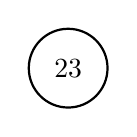
\begin{tikzpicture}[thick]
      \node[circle, draw, minimum size = 1cm]{23};
    \end{tikzpicture}
\end{minipage}\hfill
\begin{minipage}{0.6\textwidth}
    We start with an empty tree, and add our root node: $23$.
\end{minipage}

\begin{minipage}{0.4\textwidth}
    \begin{tikzpicture}[
      node distance = 1.5cm,
      level distance=1.5 cm,
      level 1/.style={sibling distance=3cm},
      level 2/.style={sibling distance=1.5cm},
      thick, minimum size=1cm]
      \node[circle,draw](23) {23}
	    child {
	    node [circle,draw](17){17}
	    }
	    child{node[circle,draw](476){476}
	    };
      \path[->, >=stealth', shorten >=1pt, auto]
	    (23) edge[bend right, blue] (17)
	    (23) edge[bend left, red] (476);
    \end{tikzpicture}
\end{minipage}\hfill
\begin{minipage}{0.6\textwidth}
    Now we add two children: $17$ and $476$.
    Clearly, $17$ becomes the left child because $17 < 23$, and $476$ become the right child because $476 > 23$.
\end{minipage}

\begin{minipage}{0.4\textwidth}
    \begin{tikzpicture}[
      node distance = 1.5cm,
      level distance=1.5 cm,
      level 1/.style={sibling distance=3cm},
      level 2/.style={sibling distance=1.5cm},
      thick, minimum size=1cm]
      \node[circle,draw] {23}
	    child {
	    node [circle,draw]{17}
	    }
	    child{node[circle,draw]{476}
		    child{node[circle,draw](28){28}}
		    child[fill=none] {edge from parent[draw=none]}
	    };
      \path[->, >=stealth', shorten >=1pt, auto]
      (23) edge[bend left, red] (476)
      (476) edge [bend right, blue] (28);
    \end{tikzpicture}
\end{minipage}\hfill
\begin{minipage}{0.6\textwidth}
    What happens if we add $28$? Starting at the root, we move to the right because $28 > 23$.
    However, there is already a right subroot there!
    $28$ must then take $476$ as its parent node and, because $28 < 476$, it is placed as the left child of $476$.
\end{minipage}

To begin writing an insertion method for our \li{BinTree} class, we consider BST's themselves.
BSTs are a recursive data structure because each of the left and right subtrees of a parent node are, themselves, BSTs.
Therefore, many of the algorithms for working with binary search trees are also recursive.
To supplement our \li{insert} method, we write a recursive function to call within our insert function:
\begin{lstlisting}
    def insert(self, data):
        def _recur_insert(node, item):
            if node == None:
                return Node(item)
           else:
               if data < node.value:
                   node.left = _recur_insert(node.left, item)
               elif data > node.value:
                   node.right = _recur_insert(node.right, item)
               else:
                   return node
            return node
\end{lstlisting}
We call this recursive function by setting it equal to the root node. 
The function will continually call itself until an empty node is found, then use \li{return node} to update each of the levels it recursively visited prior (until it returns to \li{self.root}). 
\begin{lstlisting}
        self.root = _recur_insert(self.root, item)
        self.size += 1
\end{lstlisting}


\subsection*{Finding}
Although recursive functions are often useful and intuitive with trees, we  are by no means required to use them. In fact, for large trees, a recursive algorithm will consume a lot of resources. When writing a method to search for nodes in a BST, we may either use recursion or alternate methods to ascertain whether a piece of data is, indeed, to be found within the tree.

\begin{problem}
Add a method for finding nodes to your binary tree class. If a node containing your data exists within the tree, return the node. If no such node exists, return \li{False}. 
\label{prob:BST1}
\end{problem}

\subsection*{Removing}
Removing nodes is only slightly more complicated.
We have three cases to consider:
\begin{enumerate}
\item No children.
This is the simplest case.
If the node we want to delete has no children then we simply remove the node.

\begin{minipage}{0.3\textwidth}
    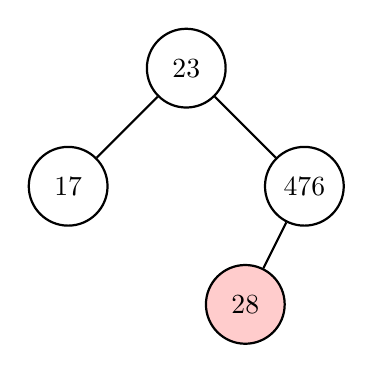
\begin{tikzpicture}[
      level distance=1.5 cm,
      level 1/.style={sibling distance=3cm},
      level 2/.style={sibling distance=1.5cm},
      thick, minimum size=1cm]
      \node[circle,draw](23) {23}
	    child {
	    node [circle,draw](17){17}
	    }
	    child{node[circle,draw](476){476}
	    	child{node[circle,draw, fill=red!20!](28){28}}
	    	child[fill=none] {edge from parent[draw=none]}
	    };
    \end{tikzpicture}
\end{minipage}
\begin{minipage}{0.2\textwidth}
   \begin{center}
     \begin{tikzpicture}[]
        \draw[->, double, double equal sign distance, -implies, thick] (0,0) -- (1.25,0);
    \end{tikzpicture}
   \end{center}
\end{minipage}
\begin{minipage}{0.3\textwidth}
    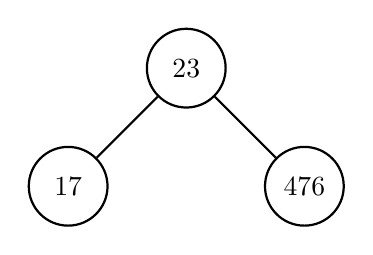
\begin{tikzpicture}[
      level distance=1.5 cm,
      level 1/.style={sibling distance=3cm},
      level 2/.style={sibling distance=1.5cm},
      thick, minimum size=1cm]
      \node[circle,draw](23) {23}
	    child {
	    node [circle,draw](17){17}
	    }
	    child{node[circle,draw](476){476}
	    };
    \end{tikzpicture}
\end{minipage}

\item One child.
In this case, we have to worry about children.
If we were to just delete the node, we would lose the entire subtree.
The solution, however, is simple enough: we promote the child to take the place of the node we are deleting.

\begin{minipage}{0.3\textwidth}
    \begin{tikzpicture}[
      level distance=1.5 cm,
      level 1/.style={sibling distance=3cm},
      level 2/.style={sibling distance=1.5cm},
      thick, minimum size=1cm]
      \node[circle,draw](23) {23}
	    child {
	    node [circle,draw](17){17}
	    }
	    child{node[circle,draw, fill = red!20!](476){476}
	    	child{node[circle,draw](28){28}}
	    	child[fill=none] {edge from parent[draw=none]}
	    };
     \path[->, >=stealth', shorten >=1pt, auto]
      (28) edge[bend left, red] (476);
    \end{tikzpicture}
\end{minipage}
\begin{minipage}{0.2\textwidth}
   \begin{center}
     \begin{tikzpicture}[]
        \draw[->, double, double equal sign distance, -implies, thick] (0,0) -- (1.25,0);
    \end{tikzpicture}
   \end{center}
\end{minipage}
\begin{minipage}{0.3\textwidth}
    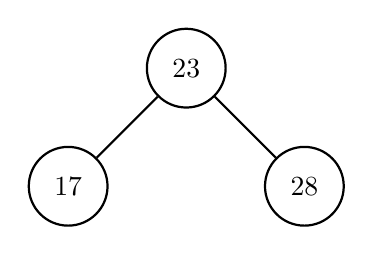
\begin{tikzpicture}[
      level distance=1.5 cm,
      level 1/.style={sibling distance=3cm},
      level 2/.style={sibling distance=1.5cm},
      thick, minimum size=1cm]
      \node[circle,draw](23) {23}
	    child {
	    node [circle,draw](17){17}
	    }
	    child{node[circle,draw](28){28}
	    };
    \end{tikzpicture}
\end{minipage}

\item Two children.
We need to be a little careful in this case.
We can't simply promote a child node.
Indeed, how would we decide which child to promote?
Fortunately, we can reduce this case down to one of the previous two cases.
Suppose we are removing node $23$, which has two children.
We first locate either the smallest node of the right subtree or the greatest node of the left subtree.
In this case, we identify node $28$ as the \emph{in order successor}: the smallest node of the right subtree.
We swap the data of nodes $28$ and $23$ (so node $28$ now has the data that $23$ had and vice versa).
Note that, because $28$ is the smallest node of the right subtree, cannot have a child to it's left, which implies it either has one child or no children.
Thus, removing $23$ has been reduced to a simpler case.

\begin{minipage}{0.3\textwidth}
\begin{tikzpicture}[
  level distance=1.5 cm,
  level 1/.style={sibling distance=3cm},
  level 2/.style={sibling distance=1.5cm},
  thick, minimum size=1cm]
  \node[circle,draw, fill = red!20!](23) {23}
	child {
	node [circle,draw]{17}
	}
	child{node[circle,draw]{476}
		child{node[circle,draw](28){28}}
		child[fill=none] {edge from parent[draw=none]}
	};	
  \node[draw=none, node distance=3cm](Note)[right of =28] {In order successor};
  \path[->, >=stealth', auto]
     (Note) edge (28)
     (23) edge[out = 5, in=15, blue, looseness=1.5] (28)
     (28) edge[bend left, red] (23);
\end{tikzpicture}
\end{minipage}
\begin{minipage}{0.2\textwidth}
   \begin{center}
     \begin{tikzpicture}[]
        \draw[->, double, double equal sign distance, -implies, thick] (0,0) -- (1.25,0);
    \end{tikzpicture}
   \end{center}
\end{minipage}
\begin{minipage}{0.3\textwidth}
    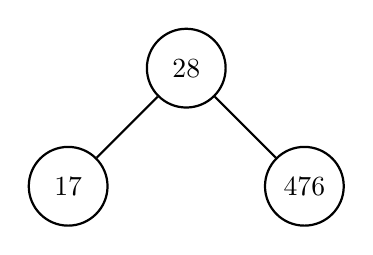
\begin{tikzpicture}[
      level distance=1.5 cm,
      level 1/.style={sibling distance=3cm},
      level 2/.style={sibling distance=1.5cm},
      thick, minimum size=1cm]
      \node[circle,draw](28) {28}
	    child {
	    node [circle,draw](17){17}
	    }
	    child{node[circle,draw](476){476}
	    };
    \end{tikzpicture}
\end{minipage}

\end{enumerate}

\begin{problem}
Give your binary tree class from Problem \ref{prob:BST1} a method for removing nodes.
Make sure  to account for all the cases given above.
\label{prob:BST2}
\end{problem}

\subsection*{Balanced Trees}
Binary search trees often perform very well in searching for data.
However, the order of insertion into a binary search tree largely determines how well the tree performs.
Binary search trees work best when elements are added in a random order.
This keeps the tree relatively full - each level has the maximum number of nodes -  rather than having some subtrees being much larger than others.
If the elements are sorted before adding to a BST, the efficiency of a BST is completely mitigated.
The resulting degenerate tree is essentially a linked list.

One method for solving these problems is to keep the tree balanced.
On each insertion and removal, the tree is re-balanced to maintain optimal performance.
AVL Trees and Red-Black Trees are examples of balanced trees.

TODO: pictures of a full tree versus adding in already sorted data.

\section*{Heaps}

A \emph{heap} is another tree-based data structure; however, heaps are only partially ordered and are always full.
This means that parents are ordered with respect to children, but unlike a BST, siblings or cousins have no order.
However, because heaps are only partially ordered, searching for nodes other than the root is not as efficient as a BST.
Heaps are commonly used for \emph{priority queues}, because the only element you need access to is the one with the greatest priority.
Max and min heaps are also common and are used when you need to find the maximum or minimum in constant time.
In a max heap, each parent is greater than its children.
This puts the maximum at the root of the tree.

%TODO: pictures of max and min heaps

To add into a heap, we put the node into an empty spot on the lowest level of the tree.
Then we compare it to its parent and if it is greater than its parent, we switch the two nodes.
We continue this until the new node reaches a parent that is greater than it or it becomes the new root.

Since heaps are really only useful for keeping track of the maximum, removing the maximum is easy, but removing anything else is not.
To remove the maximum (the root), we compare the root's children and promote the greatest to be the new root.

%TODO: pictures of insert and removing from a max heap
\begin{comment}
\section*{Sparse Matrices}
Matrices are powerful tools, but they can take a lot of space in memory.
A $n \times n$ matrix takes $n^2$ places of storage!
If every entry in the matrix is useful information this is fine, but if the matrix is filled with a lot of zeros, that means we are using almost $n^2$ spots in memory to store useless zeros.
Not only does this unnecessarily take up space, it means that during computation we will spend a lot of time adding and multiplying zeros.
That can be a lot of useless computation.
The solution to this is \emph{sparse matrices}.
They are other data structures used to represent a matrix by only storing non-zero entries.

One common way is a dictionary.
The index of the spot in the matrix is the key and the number in that spot is the value.
For example,
\[
\begin{pmatrix}
0 & 0 & 0 & 0 & 0 \\
22 & 0 & 0 & 0 & 0 \\
0 & 0 & 0 & 0 & 0 \\
0 & 0 & 5 & 0 & 0 \\
0 & 0 & 0 & 0 & -4
\end{pmatrix}
\]
would be stored as
\[
\begin{tabular}{|c|l|}
\hline
Key & Value \\
\hline
(1,0) & 22 \\
\hline
(3,2) & 5 \\
\hline
(4,4) & -4 \\
\hline
\end{tabular}
\].

In this case, we stored a 5 by 5 matrix in a dictionary with only 3 key-value pairs.

SciPy has a nice implementation of sparse matrices.
Not only does SciPy reduce the amount of space needed to store matrices, it has fast algorithms for matrix operations that takes advantage of the fact that there are so many zeros.

\begin{problem}
Use your time function from Section 1 and the code given below to time matrix multiplication using sparse matrices versus normal matrix multiplication for $ n = 100, 500, 1000, 1500,$ and $2000$. Which is faster? What happens as the matrices grow larger?
\begin{lstlisting}
from scipy import sparse
import numpy as np

#dimension of matrices
n = 100

# create 2 random sparse matrices with density 0.1
A = sparse.rand(n,n)
B = sparse.rand(n,n)

#Multiply using sparse matrix techniques
A.dot(B)

#Change to dense matrices
A_dense = A.todense()
B_dense = B.todense()

#Multiply with normal matrix multiplication
A_dense.dot(B_dense)

 \end{lstlisting}
 \label{prob:Sparse}
 \end{problem}
\end{comment}


